%!TEX root = ../dokumentation.tex

\chapter{Ordnerstruktur}
\label{ch:Ordnerstruktur}

\begin{wrapfigure}{r}{0\textwidth}
\centering
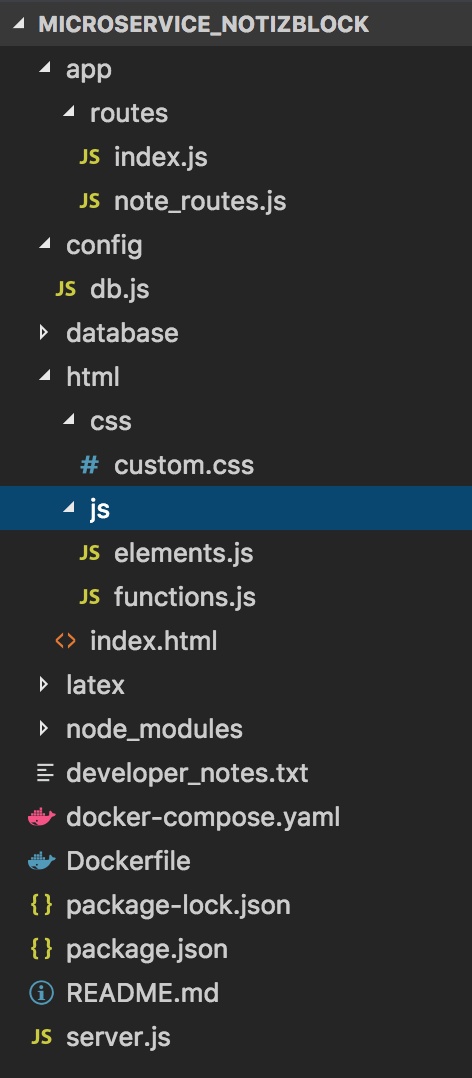
\includegraphics[height=.5\textwidth]{Ordnerstruktur.png}
\vspace{4pt}
\caption{Schaubild\footnotemark}
\label{fig:blueant}
\end{wrapfigure}

Der app-Ordner enthält die Routes der Anwendung. Diese Beschreiben die einzelnen Pfade der CRUD-Operationen.

Im config-Ordner befindet sich die db.js. Diese legt die Verbindung zur Mongo-Datenbank fest.

Der Ordner database wird für die Datenbank-Engine benötigt und enthält automatisch generierte Dateien, die mit der Installation des MongoDb-Treibers mit einher gehen.

Im html-Ordner fidnen sich alle notwendigen Dateien für die Oberfläche der Anwendung. So ist das grundlegende html-File direkt in diesem Ordner abgelegt. Das zugehörige Style-sheet befindet sich im css-Ordner, die Javascript-Methoden im js-Ordner.

Im Ordner latex befinden sich die Dateien für die Dokumentation im latex-Format.

Der Ordner node\_modules wird durch das Kommando \glqq  npm install\grqq{} und die, in der package.json festgelegten, Dependencies automatisch befüllt.

Die Datei \glqq  developer\_notes.txt \grqq{} enthält Informationen über die Pfade zu den einzelnen Methoden der Anwendung.

Das docker-compose.yaml legt die Eigenschaften der Containerorchestrierung fest. Auf diesem File beruht das spätere Kommando \glqq  docker-compose up\grqq{} das die komplette Anwendung containerisiert startet.

Das Dockerfile legt das Image des Anwendungscontainer fest.
Die package.json beschreibt die Grundlagen der Anwendung und verzeichnet die Dependencies für den Node Package Manager.
Das README wurde durch den Upload auf Github erstellt und enthält lediglich eine kurze Beschreibung der relevanten Anwendungsschnittstellen.

Die server.js-Datei bildet das Herzstück der Anwendung. Hier werden die diversen Teile der Anwendung durch Imports bzw Requirements zusammengeführt. Weiterhin wird hier der Node-Server gestartet und es werden Anforderungen für verwendete Frameworks gesetzt.